% SP manuscript in the ICS Thesis LaTeX template (icsthesis.cls)
% Build: pdflatex -> bibtex -> pdflatex -> pdflatex
\documentclass{icsthesis}
\usepackage{xurl}
\usepackage{amsmath}
\usepackage{amssymb}
\usepackage{float}
\usepackage{placeins}
\usepackage{tikz}
\usetikzlibrary{arrows.meta,positioning,shapes.geometric,arrows}

% No section numbers (the template hides them; this also keeps sub-subsections clean)
\setcounter{secnumdepth}{0}
% The template turns hyphenation off; let LaTeX stretch spacing instead of running past the margin
\setlength{\emergencystretch}{3em}
\renewcommand{\thefigure}{\arabic{figure}}
\renewcommand{\thetable}{\arabic{table}}

\renewcommand{\TITLE}{OPTIMIZING AGRICULTURAL SUPPLY CHAIN DISTRIBUTION USING MULTI-\allowbreak{}COMMODITY NETWORK FLOW MODELS}
\renewcommand{\AUTHOR}{ADRIAN CARL B. CUTINES}
\renewcommand{\DEGREE}{BACHELOR OF SCIENCE}
\renewcommand{\MAJOR}{Computer Science}
\renewcommand{\MONTH}{NOVEMBER}
\renewcommand{\YEAR}{2026}
\newcommand{\ADVISER}{JAIME SAMANIEGO}

\renewcommand{\maketitle}{
	\singlespacing
	\begin{titlepage}
	\addcontentsline{toc}{section}{TITLE PAGE}
	\begin{center}
	\vspace*{8ex}
	\invertpy{\hyphenpenalty=10000\exhyphenpenalty=10000 \TITLE}
	\vspace*{2in}
	\AUTHOR
	\\[2in]
	A SPECIAL PROBLEM SUBMITTED TO THE FACULTY OF THE\\
	INSTITUTE OF COMPUTER SCIENCE\\
	UNIVERSITY OF THE PHILIPPINES LOS BA\~{N}OS\\
	IN PARTIAL FULFILLMENT OF THE\\
	REQUIREMENTS FOR THE\\
	DEGREE OF\\
	\vspace*{.65in}
	\DEGREE\\
	(\MAJOR)\\
	\vspace*{.65in}
	\MONTH\ \YEAR
	\end{center}
	\end{titlepage}
	\doublespacing
}

\begin{document}

\begin{frontmatter}
	\maketitle

	\begin{approvalpage}
		The special problem hereto attached entitled \TITLE, prepared and submitted by \AUTHOR, in partial fulfillment of the requirements for the degree of \DEGREE\ (\MAJOR) is hereby accepted.

		\addsignature{\ADVISER}{Adviser}

		Accepted in partial fulfillment of the requirements for the degree of \DEGREE\ (\MAJOR).
		\addsignature{DR. RACHEL EDITA O. ROXAS}{Director, Institute of Computer Science}
	\end{approvalpage}

	%\begin{biosketch}
	%	[Write your biographical sketch here.]
	%	\addauthorsignaturefield
	%\end{biosketch}

	\begin{acknowledgement}
		First and foremost, I would like to give thanks to Almighty God for giving me endless grace, wisdom and strength that helped me overcome all obstacles and accomplish this project.

        I would also like to give my appreciation to my special problem adviser, Prof. Jaime M. Samaniego for giving me incredible guidance, patience and wisdom. He have given me helpful feedback and constant encouragement throughout my project.
        
        A big thank you goes to my family, parents and siblings for providing me with emotional and financial support and for being endlessly understanding.
        
        I would also like to thank my friends and peers for always being there for me. Whether it was having a coffee with you, your constant support and encouraging words made me feel uplifted. Thank you for believing in me.
        
        Lastly, I would like to thank anyone who has helped me with this study, directly or indirectly. This achievement belongs to you as well.
	\end{acknowledgement}

	\maketableofcontents
	\makelistoftables
	\makelistoffigures

	\begin{abstractwithpageno}
	\\
	\textbf{\AUTHOR}, University of the Philippines Los Ba\~{n}os, \MONTH\ \YEAR. \textbf{\TITLE}
	\\Adviser: \ADVISER\\

	With limited infrastructure, transportation costs are very high in Philippine agriculture. This study formulates an optimization problem using a Capacitated Multi-Commodity Network Flow (MCNF) model to optimally distribute palay (milled rice equivalent) and corn from 15 supply nodes in various provinces in Regions I, II and III to demand nodes in the provinces and Metro Manila (NCR). A MCNF model was developed using Pyomo and solved using GLPK. NetworkX was used to visualize the optimal network. The total cost of the system was reduced by 35.68\% through optimization compared to a greedy algorithm based Business-as-Usual (BAU) solution that respects the capacity constraints. Demand fulfillment was increased to 98.41\% from 93.21\%. This means that the transportation costs were reduced by 2.23\%, with 96.6\% of the savings coming from reduction in demand shortages. The remaining 1.59\% of demand is unmet, at Bataan and Zambales. It persists even with unlimited arc capacity, so, within the modeled network, it is caused by missing supply links rather than saturated roads. The most utilized arc is from Nueva Ecija\_S to Bulacan\_S with 100\% utilization, followed by Isabela\_S to Nueva Ecija\_S with 99.68\%. Capacity limits increase the optimal cost by 1.97\%, and unmet demand remains at 1.59\% until capacity falls to 60\% of its base value.

	\noindent\textbf{Keywords:} Agricultural supply chain, Multi-Commodity Network Flow (MCNF), logistics optimization, distribution efficiency, post-harvest loss, Pyomo, GLPK, NetworkX
	\end{abstractwithpageno}
\end{frontmatter}

\begin{mainmatter}
\section{INTRODUCTION}
Agriculture supply chains are a key part of transporting produce efficiently from producers to consumers. However, there are issues with agricultural supply networks such as high transport costs, poor infrastructure and post-harvest losses. Common resource allocation methods and routes are also not reflective of the complexities involved with transporting various types of produce and using a joint transport method.

Efficient logistics and data in the agriculture industry is essential to ensure food is supplied efficiently, particularly when transporting perishable products where quick delivery can be a key issue. As the complexity of the agriculture industry increases alongside fluctuating supply and demand there has been an increased need for data driven models. Inefficiencies in the distribution system cause financial issues for farmers, suppliers and consumers and less product being available will affect the income and food availability.

By using Network Flow Algorithms we can provide a systematic way of solving these problems. Multi-Commodity Network Flow (MCNF) enables us to manage multiple goods (such as Palay and Corn) with separate supply and demand constraints by simultaneously transporting them in the same network. MCNF helps us to satisfy the demand for each good whilst accounting for transport constraints to reduce overall impacts on costs.

This can be applied to agriculture allowing us to quantify the trading of limited transport capacity between commodities. MCNF indicates how the specific demand of products interacts with the shared network. This allows us to identify the methods to find the most efficient and least costly point. Furthermore it represents a step towards creating digital and automated tools that can help decision makers (Policymakers, Transport Managers and Agricultural Cooperatives) by providing them with up to date information.

This study uses MCNF in an agricultural supply chain to demonstrate how optimisation techniques can improve distribution efficiency, reduce wastage and identify areas of bottlenecking within the logistics network. It is anticipated that the results will provide tangible solutions to agricultural planning issues as well as contribute to academic literature by quantifying the optimisation of a multi-commodity network.

This issue is being tackled by using mathematical modelling. This study can contribute to agricultural logistics and food distribution. The results obtained from the study could prove to be key in guiding future policy and investment decisions especially within rural areas that are underdeveloped and lack transport infrastructure. This work aims to demonstrate that optimisation algorithms can be implemented within agricultural systems to bridge the gap between research and real world applications, making the supply chain network more robust and cheaper.

% STATEMENT OF THE PROBLEM
\subsection{Statement of the Problem}
The agricultural supply chain in the Philippines suffers from many inefficiencies, such as high logistics costs, poor infrastructure, and considerable wastage after harvest. The difficulties are aggravated when dealing with multiple commodities in a single supply chain system because different commodities like palay and corn vie for scarce resources. The present system does not have the optimization needed to ensure efficient use of resources, thus causing high costs and wastage of food products.

\begin{enumerate}
    \item Lack of Network Formalization: There does not exist a standard mathematical notation of agricultural logistics chain networks to facilitate the application of computational algorithms for detecting network inefficiencies.
    \item  Inefficient Multi-Commodity Management: Current approaches do not take into consideration the combined movement of different goods, causing large amounts of transportation inefficiencies due to overburdened vehicles.
    \item Quantification of Logistical Waste: Furthermore, there is a lack of empirical evidence regarding the reduction of logistical waste from an optimization standpoint; logistical waste refers to waste created due to capacity limitations rather than spoilage.
\end{enumerate}

This study addresses the following central question: \textit{How can Multi-Commodity Network Flow models optimize agricultural distribution to reduce costs, minimize logistical waste, and improve resource allocation across the supply chain?}


\subsection{General Objective}
To optimize the distribution of agricultural products using multi-commodity network flow models, ensuring cost efficiency, reduced logistical waste, and balanced allocation of resources across the supply chain.


\subsection{Specific Objectives}
\begin{enumerate}
\item Network Modeling: To construct an agricultural supply chain as a directed network graph, comprised of nodes representing sources (provincial farm supply), transshipment points (supply nodes that relay goods), and sinks (cities).
\item Multi-Commodity Integration: To simulate the flow of different types of commodity (palay and corn) in a network using one system but subject to capacity constraints on edges as well as individual demand curves.
\item System Evaluation and Waste Analysis: To quantify improvements in cost-efficiency and supply utilization by comparing optimized flows against a Business-as-Usual (BAU) baseline, and to identify bottlenecks and quantify logistical waste.
\end{enumerate}

% SIGNIFICANCE OF THE STUDY
\subsection{Significance of the Study}
The findings of this study will provide valuable insights for:

\textbf{Farmers:} Making sure that the products are delivered on time and that the income is potentially increased as a result of lower post-harvest losses.

\textbf{Transport and Logistics Companies:} Improving the usage of vehicles and facilitating planning of routes that are more efficient.

\textbf{Policymakers and Cooperatives:} Providing data-backed assistance for the choices regarding agricultural infrastructure and logistics investments.

\textbf{Academic Community:} Helping with research on mathematical optimization and the use of multi-commodity network flow models in the context of developing countries.

By demonstrating the effectiveness of MCNF in agricultural supply chains, this study helps bridge the gap between theoretical models and practical logistics solutions.

% SCOPE 
\subsection{Scope of the Study}
This study focuses on the optimization of agricultural supply chain distribution using Multi-Commodity Network Flow (MCNF) models. Specifically, it includes:

\begin{itemize}
    \item Modeling agricultural supply chains as networks of supply nodes (farms, which may also act as transshipment hubs) and demand nodes (markets); dedicated warehouse nodes are not included.
    \item Optimizing the simultaneous flow of multiple commodities with distinct supply and demand requirements through shared transportation networks.
    \item Evaluating improvements in distribution efficiency, transportation cost reduction, and potential reduction of post-harvest losses.
    \item Using computational tools such as Pyomo, GLPK, and NetworkX for modeling, optimization, and visualization of commodity flows.
    \item Representing the principal north-to-south freight corridor toward Metro Manila as a network of 20 inter-province arcs, plus one local distribution arc per province.
\end{itemize}

The study does not consider weather, climate variability, natural disasters, or other environmental and socioeconomic influences, except that road disruptions (e.g., typhoon closures) are simulated as proportional reductions in arc capacity. The study is restricted to network-based optimization driven by supply, demand, transportation capacity and cost. Perishability is not modeled; the two commodities studied, palay and corn, are not cold-chain goods.

% DEFINITION OF TERMS
\subsection{Definition of Terms}

\textbf{Agricultural Supply Chain} – The sequence of processes involved in producing, transporting, storing, and distributing agricultural products from farms to markets.

\textbf{Multi-Commodity Network Flow (MCNF)} – An optimization model that supports the simultaneous movement of multiple commodities through a shared network while satisfying supply, demand, capacity, and cost constraints.

\textbf{Commodity} – A distinct type of agricultural product (e.g., palay, corn) with its own supply, demand, and perishability characteristics.

\textbf{Supply Node} – A point in the network where agricultural products originate, typically representing farms or production areas.

\textbf{Demand Node} – A point in the network where products are needed or consumed, usually markets or distribution centers.

\textbf{Intermediate Node} – A storage or transit point within the supply chain network, such as a warehouse or consolidation facility.

\textbf{Network Flow} – The mathematical representation of commodity movement through interconnected nodes and routes (arcs) within a logistics network.

\textbf{Transport Capacity} – The maximum quantity of goods that can be transported along a specific route or by a particular vehicle.

\textbf{Perishability} – The tendency of agricultural goods to spoil or degrade over time, requiring timely and efficient transportation.

\textbf{Post-Harvest Losses} – The reduction in quantity or quality of agricultural products after harvest due to delays, poor handling, or inadequate distribution systems.

\textbf{Logistical Waste} – Supply that stays unused at source nodes because arc capacities prevent it from reaching demand, measured as the extra unmet demand of the capacitated model over the uncapacitated model. Unused supply in excess of total demand is reported separately as structural surplus.

\textbf{Optimization} – A mathematical method used to identify the most efficient allocation of resources, usually by minimizing cost or waste while satisfying constraints.

\textbf{Routing} – The process of selecting optimal transportation paths from supply nodes to demand nodes.

\textbf{Logistics Efficiency} – The effective use of time, resources, and transportation capacity to minimize cost and waste in the distribution system.

\textbf{Resource Allocation} – The method of distributing limited resources such as transport capacity or storage space among multiple commodities.

\textbf{Computational Modeling} – The use of algorithms and software tools (e.g., Pyomo, GLPK) to simulate, analyze, and optimize complex logistics networks.

\textbf{Cold Chain Logistics} – A temperature-controlled supply chain system essential for transporting perishable goods such as fish, vegetables, and fruits.

\textbf{Baseline Scenario} – A reference model representing non-optimized or traditional distribution practices used to compare improvements from the MCNF model.

\textbf{Network Visualization} – The graphical representation of a logistics network using tools like NetworkX to display nodes, routes, and optimized commodity flows.


% MATERIALS AND METHODS
\section{REVIEW OF RELATED LITERATURE}


\subsection{Related Literature}
Agricultural logistics has been relying increasingly on optimization models to improve efficiency. Among these, a promising model is the Multi-Commodity Network Flow (MCNF). The MCNF model can be applied to several fields, such as logistics, telecommunications and energy distribution. Recently, it was applied to agri-food supply chains to better coordinate different aspects and reduce costs.


\subsubsection{Network Flow Models in Agriculture}
These studies show how MCNF can be used to model these interrelated flows of different agricultural products within the supply chain. A study conducted by \citet{ahumada2009}, showed that mathematical planning models can significantly reduce loss and costs (perishable). The results of another study concluded that perishability is highly influential on design and management of agri-food supply chains \citep{esteso2021}. This therefore shows that time based tools are an important aspect. Overall all articles agree that multi-commodity network flow models can be used as a tool to optimise the loss during operations due to the complex nature of agricultural logistics, plus also the overall cost.


\subsubsection{Perishability and Time-Sensitive Logistics}
One of the major challenges in the field of agriculture logistics is handling perishables. The distribution of perishables (fruits, vegetables, fish, meat etc.) must be done in a timely and efficient manner. Including perishables within supply chain models will allow for the simulation of transit times and identification of bottlenecks in the system. This can be achieved by using MCNF and other computational methods \citep{esteso2021}.

This study does not consider perishables. Palay and corn are not cold chain goods. However, capacity constraints can still be included to account for delays in deliveries. Time sensitive spoilage will be considered in future work.


\subsubsection{Applications in Developing Countries}
Logistics inefficiencies, supply chain fragmentation, and poor infrastructure of a developing economy such as in the Philippines can be used as a basis for developing optimization models. According to \citet{pids2017}, the agricultural sector suffers from high distribution costs and loss of product due to persistent issues in the transport, handling, and post-harvest losses of products. The same idea is being hypothesized by \citet{briones2022} in their study on how modernization of agricultural value chains can be achieved by improving logistics planning, and through the use of digital and optimization tools to improve overall efficiency. However, according to \citet{adriano2022}, inefficiencies in the supply chain structure, high production costs, and poor integration results in very little value being captured by the producers in the Philippines agricultural value chains. These studies form the basis of highlighting the importance of using optimization models such as MCNF to aid effective planning and equitable distribution of value in the value chain.


\subsubsection{Synthesis and Research Gap}
There is a wide body of literature that shows optimization and network flow models are important in the field of agricultural logistics, but they have not been widely implemented. Literature surrounding the difficulties of transporting multiple different goods within the limited infrastructure of developing countries has also not been widely explored.

Most literature focuses upon the biological causes of food loss. To our knowledge, little literature estimates the losses due to logistical issues, that is, the amount of goods stuck at their source because of logistical problems. Previous models have often not considered the trade-off between the cost of transport and market penalty in areas with poor logistical infrastructure.

In this study, an MCNF model will be used to tackle these issues, taking into account the geographical conditions of the Philippines. A transshipment formulation will be used in this research.

%APPLICATIONS
\subsection{Applications} 
The multi-commodity network flow (MCNF) model can be applied to several agricultural logistics tasks:


\subsubsection{Crop Distribution}
For instance, the model can support the transportation of key crops (e.g. rice and corn) from surplus areas to areas of high demand through reducing the transportation costs. This allows for the most optimal allocation of the available transport capacity and ensures that supply and demand are balanced between different regions.


\subsubsection{Cold Chain Logistics}
MCNF can be used in the optimization of the cold chain logistics. This type of optimization is necessary when transporting perishable goods, such as fish, vegetables, and fruits. The model will identify the most efficient way of utilizing the limited cold storage and refrigerated transport facilities decreasing the amount of spoilage and increasing the quality.


\subsubsection{Disaster Relief Logistics}
The MCNF can be used to help logistics planning during emergency situations, such as quickly distributing relief supplies, for example, rice, canned goods and bottled water, to people affected by natural disasters. It can be used to determine what routes will deliver goods to people in the cheapest and fastest way by considering capacity, demand and cost constraints.


\subsubsection{Export and Trade Logistics}
Using the MCNF model, these agricultural systems can be optimized for export oriented. It can help optimize international trade of goods such as bananas, coconut by-products, pineapple to various production areas and ports throughout the Philippines before exporting to various areas in the world. This helps improve trade logistics, reduce costs, and give agricultural exports an advantage in the market.



Overall, these applications illustrate the adaptability of the MCNF model to a wide range of agricultural and humanitarian contexts, making it a valuable tool for addressing logistical and policy challenges.

%Software Tools
\subsection{Software Tools}
To put MCNF models into action, you need computational tools that can handle the massive optimization problems very efficiently. There are some open-source as well as commercial software platforms that have been designed for this task, such as:


\subsubsection{Python OR-Tools (Google)}
A cutting-edge open-source optimization suite by Google, OR-Tools provides not just but very robust solvers for both linear programming and minimum-cost flow problems. Moreover, it is perfect for large-scale MCNF implementations that require multiple commodities and transport modes. OR-Tools was reviewed as an alternative solver interface but was not used in this study; the model is implemented in Pyomo and solved with GLPK.


\subsubsection{Pyomo}
Pyomo is a powerful optimization modeling language in Python that is capable of not only creating but also solving intricate optimization problems. Furthermore, it supports the integration of perishability, capacity, and cost constraints, thus being very adaptable to the analysis of agricultural network flow.


\subsubsection{NetworkX}
A Python-based package that can be used to create, visualize, and analyze the structure of networks. Specifically in agricultural logistics, NetworkX can illustrate the connections among farms, warehouses, and markets and can be integrated smoothly with OR-Tools or Pyomo for simulation and optimization.



The proposed tools, when used together, will provide a computational framework that is not only flexible but also very useful for modeling MCNF-based agricultural logistics systems, thus facilitating both theorems and real-life distribution planning applications.


% Methodology
\section{THEORETICAL FRAMEWORK, METHODOLOGY, AND SYSTEM DESIGN}

%Theoretical Framework
\subsection{Theoretical Framework}
This study is based on Network Flow and Optimization theory, used to model and solve complex logistics problems. Within the agriculture industry, multiple types of product will use the same routes to transport, therefore it is essential to optimise the networks flows to reduce costs, reduce wastage, and improve resource usage.

The multi-commodity network flow (MCNF) formulation is a well-known network optimization model \citep{ahuja1993}, and has been used by \citet{rodrigo2018} for multi-commodity transportation. This model allows the different commodities to flow optimally along the same routes, whilst ensuring the supply, demand, and capacity constraints are maintained for each commodity. This can be applied within the agriculture industry by designing a network containing the farms, warehouses and markets as nodes, with arcs representing the transportation links.


\subsubsection{Network Flow Theory}
Network Flow Theory represents the movement of commodities through a system of nodes and arcs.
\textbf{Supply nodes:} farms or production centers.
\textbf{Intermediate nodes:} warehouses or storage facilities.
\textbf{Demand nodes:} markets or distribution centers.

The MCNF model takes this framework a step further by addressing the issues of multiple commodities which have different supply and demand and also flow specifications. Moreover, the network can be shared by each commodity; however, it will have to comply with the individual constraints e.g. storage requirements, and vehicle capacity \citep{rodrigo2018}.


\subsubsection{Optimization Theory}
Optimization theory provides the required base to discover the most efficient flows in the network.

The MCNF model aims to minimize the total cost of transport in the most effective way possible by assuring that demand is satisfied and supply not exceeded, along with not surpassing the capacities of the routes.

In other words, the model determines the flow of commodities through each route so that the total transportation costs are minimized while all logistical constraints are satisfied.

This description follows the same structure used by \citet{rodrigo2018}.


%CONCEPTUAL FRAMEWORK   
\subsection{Conceptual Framework}

This study conceptualizes the agricultural supply chain as a multi-commodity flow network consisting of nodes (farms, warehouses and markets) and arcs (transport). The optimization model takes into account supply, demand and capacity. The MCNF model is used to find the optimal flows which minimize the total transportation cost and satisfy the constraints. This results in an improvement in the commodity paths, reduction in cost and key performance indicators of the network aiding logistics planning and decisions.

\usetikzlibrary{shapes.geometric, arrows}

\begin{figure}[htbp]
\centering
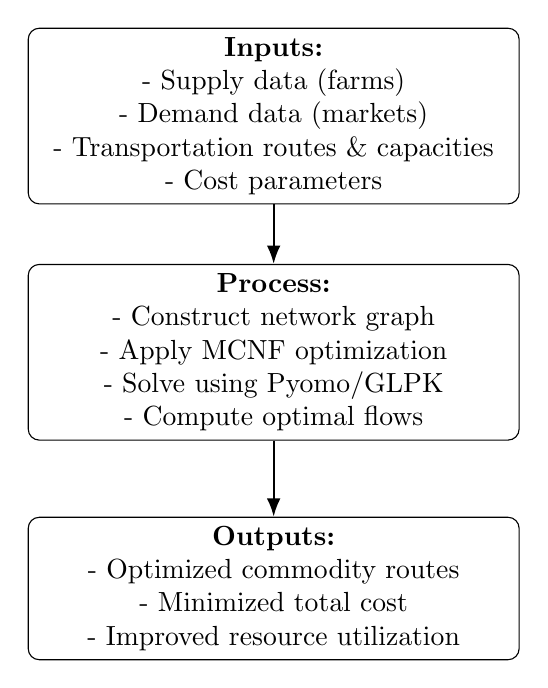
\begin{tikzpicture}[node distance=3cm]

\node (input) [rectangle, rounded corners, draw, text width=6cm, align=center] {
\textbf{Inputs:} \\
- Supply data (farms) \\
- Demand data (markets) \\
- Transportation routes \& capacities \\
- Cost parameters
};

\node (process) [rectangle, rounded corners, draw, text width=6cm, align=center, below of=input] {
\textbf{Process:} \\
- Construct network graph \\
- Apply MCNF optimization \\
- Solve using Pyomo/GLPK \\
- Compute optimal flows
};

\node (output) [rectangle, rounded corners, draw, text width=6cm, align=center, below of=process] {
\textbf{Outputs:} \\
- Optimized commodity routes \\
- Minimized total cost \\
- Improved resource utilization
};

% Draw arrows between boxes
\draw[thick, ->, >=Latex] (input.south) -- (process.north);
\draw[thick, ->, >=Latex] (process.south) -- (output.north);


\end{tikzpicture}
\caption{IPO Model for Optimizing Agricultural Supply Chain Using MCNF}
\label{fig:ipo_model}
\end{figure}




% METHODOLOGY
\subsection{Methodology}
A computational quantitative approach has been taken in this study. The formulation of MCNF as used by \citet{rodrigo2018} has been modified to apply to agricultural supply chains.


\subsubsection{Data Collection}
Data were collected to ensure the study can be replicated. Supply, population, and consumption data were taken from the sources cited below, and arc data were derived from road distances as described in the Spatial and Infrastructure paragraph. Data were grouped into three main categories:

\textit{Production and Supply Parameters:} The data on the provincial level production of palay and corn ($s_i^k$) across 15 supply nodes in Regions I, II, and III were sourced from the Philippine Statistics Authority (PSA) OpenSTAT database \citep{psa2025openstat}. The overall supply is 8,141,509 t (palay (milled rice equivalent) = 5,367,447 t; corn = 2,774,062 t).

\textit{Spatial and Infrastructure Data:} The network has 35 arcs: 20 inter-province arcs and 15 local arcs linking each province's supply node to its own demand node. Each inter-province arc has a road distance, a cost per ton, and an annual capacity (Appendix A). Cost per ton is computed as
\[
c_{ij} = d_{ij} \times \frac{\text{trip cost per km}}{\text{truck capacity}} = d_{ij} \times \frac{60}{20\ \text{t}} = 3\, d_{ij},
\]
where $d_{ij}$ is the road distance in km. The transport cost per km of 60 and the truck capacity of 20t have been assumed. These values match available data on on-demand truck pricing where prices range from 50-85 per extra km for 6-wheeler and 10-wheeler wing vans with a 12--28t capacity \citep{transportify2026}. Changing the price per km between 50-85 means the cost difference between BAU will vary between 35.5\% and 35.9\%. Unmet demand and saturated arcs remain the same.

Annual capacities $u_{ij}$ are assumed corridor capacities expressed in tons per year; each corresponds to roughly 40 to 300 truck trips per day of 20 t (capacity $\div$ ($20 \times 365$)). Local arcs have an assumed cost of 20 per ton and effectively unlimited capacity (99,000,000), because distribution within a province is outside the scope of this study.

PSA reports palay production as unmilled palay; it was converted to milled rice equivalent using the PSA milling recovery rate of 63\% \citep{usda2025}, so that rice supply and demand are in the same unit.

\textit{Market Demand Profiles:} Demand at each node is human food consumption, computed as
\[
d_i^k = \frac{\text{Population}_i \times c^k}{1000}\quad \text{(t/yr)},
\]
where $c^k$ is the annual per capita consumption in kg: 118 kg of milled rice \citep{da2020} and 15 kg of corn \citep{pcaf2023}. Provincial populations are from the PSA city and municipality population projections \citep{psa2025pop}, and the Metro Manila population is from \citet{macrotrends2025}. Demand was computed before optimization and supplied to the application as an input file; the populations and resulting demands are listed in Appendix B. Total demand is 5,017,732 t (rice 4,451,822 t; corn 565,910 t). Animal feed and industrial uses are not included.


\subsubsection{Network Scope and Arc Selection}
The model uses a subset of arcs linking the provinces: specifically, 20 arcs forming the main route of goods movement from the northern provinces (Regions I and II) through Region III and into Metro Manila. There are other roads between some provinces, for example between Isabela and Bulacan, and Tarlac and Zambales but have been omitted in order to keep the case study simple and results interpretable. As such, the optimal route will be between the arcs included in the model, and not those not included. Note that adding arcs cannot increase the optimal cost. Therefore results are dependent upon the choice of network. The size of the saving relative to the baseline may differ in a more complete road network.


\subsubsection{Model Formulation}
The model was developed to reflect the structure of the agricultural supply chain. A network structure was created consisting of nodes (farms, markets) and arcs (transport links). The supply, demand and flows for each commodity were also specified.

The objective function minimises the overall transport costs whilst accounting for supply and capacity constraints. Penalty costs are included to account for unmet demand \citep{rodrigo2018}.

A transshipment formulation was used so that goods can be consolidated and relayed through provincial supply nodes acting as hubs (e.g., Nueva Ecija\_S and Bulacan\_S in Region III).

In this case study there are no separate warehouse nodes; provincial supply nodes serve as the transshipment hubs, so the intermediate-node conservation constraint is included for generality but is inactive.

The model has been compared to a Business-as-Usual (BAU) scenario using a greedy heuristic. Palay will be transported first. Each commodity will be sent to the demand node with the largest demand first, sourced from the cheapest farm available via their Dijkstra shortest path. Once the arc capacity has been reached the arc will no longer be available. The BAU accounts for the capacities on the arcs however doesn’t optimise the flows between commodities or demand nodes. This shows different logistics actors acting independently to their own local costs.

Scenario Multipliers have been included within the implementation to analyse the resilience of the network. This allows the Northern Luzon Food Corridor to be stress tested with different harvest yields and capacity constraints.


\subsubsection{Computational Implementation}
The model will be implemented using:

Pyomo: for mathematical modeling and optimization using Linear Programming (LP).

GLPK Solver: for solving the LP-based network flow problem and computing optimal flows.

NetworkX: for visualization of network flows and optimization results.

The Sensitivity Analysis module has been implemented such that the Penalty Multiplier ($\lambda$) and Capacity Scaling Factors can be varied. This allows the user to simulate infrastructure failures for example roads being closed due to a typhoon and changes to the economic factors such as fuel price.

This setup ensures efficient computation and visual representation of multi-commodity flows across the agricultural network.


\subsubsection{Model Evaluation}
Model performance is evaluated based on the following metrics:

\begin{itemize}

    \item \textbf{Cost Efficiency:} \\
    The total system cost includes both transportation cost and penalty for unmet demand:
    \[
    \text{Total Cost} = 
    \sum_{k \in K} \sum_{(i,j) \in A} c_{ij} \cdot x_{ij}^k 
    + \sum_{k \in K} \sum_{i \in N} P \cdot u_i^k
    \]
    where $u_i^k$ represents unmet demand and $P$ is the penalty cost per unit. 
    This is compared against the baseline (BAU routing).

    \item \textbf{Demand Satisfaction:} \\
    Measures how much demand is fulfilled across all demand nodes:
    \[
    \text{Demand Satisfaction Rate} = 
    \frac{\text{Total Demand} - \text{Total Unmet Demand}}{\text{Total Demand}}
    \]

    \item \textbf{Supply Utilization:} \\
    Indicates how effectively available supply is distributed:
    \[
    \text{Supply Utilization} = 
    \frac{\sum_{k \in K}\sum_{i \in N_s}\Big(\sum_{j:(i,j)\in A} x_{ij}^k - \sum_{j:(j,i)\in A} x_{ji}^k\Big)}{\text{Total Available Supply}}
    \]
    Net outflow (outflow minus inflow) is used so that goods relayed through supply nodes acting as hubs are not counted twice.

    \item \textbf{Capacity Utilization (Edge-Level):} \\
    Evaluates how much of each route's capacity is used:
    \[
    \text{Utilization}_{ij} = 
    \frac{\sum_{k \in K} x_{ij}^k}{u_{ij}}
    \]
    This metric is used for bottleneck analysis.

\end{itemize}


The Baseline Scenario (Business as Usual) is the capacity respecting greedy shortest path heuristic described in the Model Formulation subsection. The difference between the optimised model and baseline gives an indication of the efficiency gain achieved due to coordinated routing.

These metrics have been adapted from \citet{rodrigo2018}. Demand satisfaction and unmet demand has been given more focus.



%System Design
\subsection{System Design}
The proposed system has three layers:

\subsubsection{Data Input Layer}
Accepts supply, demand, transportation, and commodity data.
Stores data in structured formats (CSV or database).

\subsubsection{Optimization Engine}
Implements the MCNF model using Pyomo and the GLPK solver.
Solves for optimal flows under supply, demand, and capacity constraints.

\subsubsection{Output \& Visualization Layer}
Generates maps of commodity flows using NetworkX.
Displays optimized routes, total cost, and flow summaries.


The system allows interactive scenario testing through a Streamlit interface, enabling adjustments to parameters such as supply, demand, transportation capacity, and penalty multiplier.

The Output Layer performs Bottleneck Detection by calculating the edge utilization ratio ($\frac{\sum \text{flow}}{\text{capacity}}$). It visually categorizes road segments into 'Critical' ($\ge 90\%$) and 'Warning' ($\ge 70\%$) zones using heatmaps generated via NetworkX and Matplotlib.

\subsection{Multi-Commodity Network Flow (MCNF) Model}

The Multi-Commodity Network Flow (MCNF) problem was defined on a directed network 
$G = (N, A)$, where $N$ is the set of nodes and $A$ is the set of arcs. Let $K$ denote the set of commodities.

Each commodity $k \in K$ is associated with:
\begin{itemize}
    \item Supply at supply nodes
    \item Demand at demand nodes
    \item Transportation cost $c_{ij}$ on each arc $(i,j)$
\end{itemize}

\textbf{Decision Variables:}
\[
x_{ij}^k = \text{flow of commodity } k \text{ on arc } (i,j)
\]
\[
u_i^k = \text{unmet demand of commodity } k \text{ at node } i
\]

\textbf{Objective Function:}
\[
\min \sum_{k \in K} \sum_{(i,j) \in A} c_{ij} \cdot x_{ij}^k 
+ \sum_{k \in K} \sum_{i \in N} P \cdot u_i^k
\]
where $P$ is the penalty cost per unit of unmet demand.

\textbf{Constraints:}

\textit{Supply Constraint:}
\[
\sum_{j:(i,j)\in A} x_{ij}^k - \sum_{j:(j,i)\in A} x_{ji}^k \le s_i^k, 
\quad \forall i \in N_s, \; k \in K
\]

\textit{Demand Constraint:}
\[
\sum_{j:(j,i)\in A} x_{ji}^k + u_i^k = d_i^k, 
\quad \forall i \in N_d, \; k \in K
\]

\textit{Flow Conservation (Intermediate Nodes):}
\[
\sum_{j:(i,j)\in A} x_{ij}^k = \sum_{j:(j,i)\in A} x_{ji}^k, 
\quad \forall i \in N \setminus (N_s \cup N_d), \; k \in K
\]

\textit{Arc Capacity:}
\[
\sum_{k \in K} x_{ij}^k \le u_{ij}, \quad \forall (i,j) \in A
\]

\textit{Non-negativity:}
\[
x_{ij}^k \ge 0, \quad u_i^k \ge 0
\]

Supply nodes may also relay goods from other supply nodes, so the supply constraint limits net outflow (outflow minus inflow) to the local supply $s_i^k$.

\textit{Discussion of Model Parameters:}

\textit{1) Shortage Penalty and Food Security Prioritization:} This penalty can be calculated as: $ P = C_{\max} \times \lambda $. Where $ C_{\max} $ is the maximum cost of supply to demand for any route in the network (i.e. the longest route at 2,040 cost units). $ \lambda $ is an arbitrary scaling factor defined by the user (default value is 2.0). The resulting penalty is therefore $ P = 4{,}080 $ per unmet tonne. As this is higher than any possible delivery route, the solver will never choose to have shortages rather than a feasible solution. Our model will only enter a shortage state $ u_i^k > 0 $ if the delivery is physically impossible. For all values of $\lambda$ tested between 1.1 and 3.0, unmet demand remained constant at 1.59\%. The total cost saving relative to BAU, however, depends on $\lambda$ (25.30\% at $\lambda=1.1$ to 43.20\% at $\lambda=3.0$) because most of the saving is avoided penalty.

\textit{2) Quantification of Logistical Waste (Objective 3):} Unused supply at a source node is
\[
W_i^k = \max\left(0,\; s_i^k - \Big(\sum_{j:(i,j)\in A} x_{ij}^k - \sum_{j:(j,i)\in A} x_{ji}^k\Big)\right).
\]
The total supply (8.14M t) is greater than the total food demand (5.02M t) by 38.37\%; thus there is a structural surplus of supply over food demand. Corn has the largest surplus with it having a supply of 2.77M t while only having a demand of 0.57M t. The uncapacitated model has a remaining demand of 79,726.57t, similar to the capacitated model. This means that there is no shortage due to capacity at the baseline capacity (0 t). The unmet demand in Bataan and Zambales arise due to there being no incoming arcs from surplus provinces. While the model does not experience shortages due to capacity, there are increased costs. The optimal solution with capacity constraints had increased costs by 38,385,894 cost units (1.97\%).

\textit{3) Continuous Flow Assumption:} The model is formulated as a Linear Programming (LP) problem with continuous variables. It assumes that agricultural commodities are divisible (measured in metric tons) and that transport occurs in a steady state:$$x_{ij}^k \in \mathbb{R}^+$$This ensures computational efficiency when simulating large-scale multi-commodity flows across the target regions and the NCR.

\textbf{Discussion:}  
The model was expressed as a Linear Programming (LP) model where continuous variables of flow were used. The MCNF model was extended to include unmet demand variables in order to overcome infeasible demands. Penalty costs were added to these variables to ensure that the overall cost was minimised.

\subsection{Illustrative Example: Shared Capacity Between Commodities}
To illustrate how the MCNF model allocates shared capacity, a small network was solved with the same application. One farm (CentralFarm\_S) supplies 50 t of rice and 50 t of corn to two markets: RiceMarket\_D (50 t of rice) and CornMarket\_D (50 t of corn). Goods can travel through a warehouse (MainHub\_W) or directly to each market (Table~\ref{tab:toy_edges}, Fig.~\ref{fig:toy}). The arc into the warehouse costs 1 per ton but can carry only 50 t in total, which is enough for one commodity but not both. The direct routes cost 2 per ton for rice and 10 per ton for corn.

\begin{table}[H]
\caption{Arcs of the illustrative network}
\label{tab:toy_edges}
\centering
\small
\setlength{\tabcolsep}{3pt}
\begin{tabular}{llrr}
\hline
From & To & Cost (/t) & Capacity (t) \\
\hline
CentralFarm\_S & MainHub\_W & 1 & 50 \\
MainHub\_W & RiceMarket\_D & 0 & 1,000 \\
MainHub\_W & CornMarket\_D & 0 & 1,000 \\
CentralFarm\_S & RiceMarket\_D & 2 & 1,000 \\
CentralFarm\_S & CornMarket\_D & 10 & 1,000 \\
\hline
\end{tabular}
\end{table}

\begin{figure}[H]
\centering
\resizebox{0.85\textwidth}{!}{%
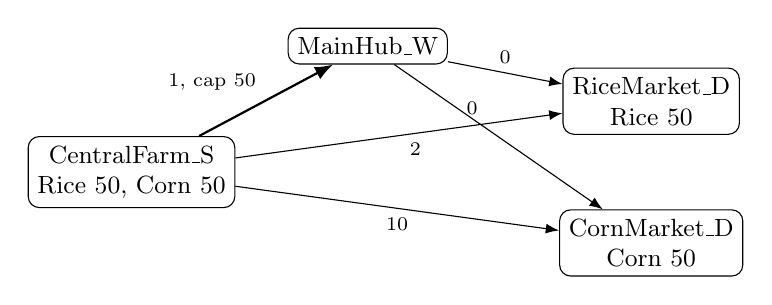
\begin{tikzpicture}[>=Latex,
  every node/.style={draw, rounded corners, align=center, font=\small}]
\node (F) at (0,0) {CentralFarm\_S\\Rice 50, Corn 50};
\node (H) at (3,1.6) {MainHub\_W};
\node (R) at (6.6,0.9) {RiceMarket\_D\\Rice 50};
\node (C) at (6.6,-0.9) {CornMarket\_D\\Corn 50};
\draw[->, thick] (F) -- node[draw=none, above left, font=\scriptsize]{1, cap 50} (H);
\draw[->] (H) -- node[draw=none, above, font=\scriptsize]{0} (R);
\draw[->] (H) -- node[draw=none, right, font=\scriptsize, pos=0.3]{0} (C);
\draw[->] (F) -- node[draw=none, below, font=\scriptsize, pos=0.55]{2} (R);
\draw[->] (F) -- node[draw=none, below, font=\scriptsize]{10} (C);
\end{tikzpicture}}
\caption{Illustrative network. Arc labels show cost per ton; the warehouse arc is limited to 50 t.}
\label{fig:toy}
\end{figure}

The greedy BAU heuristic routes rice first along its cheapest path, through the warehouse, which fills the 50 t warehouse arc. Corn must then use its direct route at 10 per ton, for a transport cost of $50(1) + 50(10) = 550$. The MCNF model considers both commodities together. It sends corn through the warehouse and rice directly, for a cost of $50(2) + 50(1) = 150$, which is 72.7\% lower (Table~\ref{tab:toy_results}). The model gives the scarce capacity to the commodity whose alternative route is most expensive, even though rice alone would also prefer the warehouse. Both plans meet all demand. The flow through MainHub\_W also shows the intermediate-node conservation constraint at work: the 50 t of corn entering the warehouse equals the 50 t leaving it.

\begin{table}[H]
\caption{Illustrative example: BAU vs.\ MCNF}
\label{tab:toy_results}
\centering
\small
\setlength{\tabcolsep}{3pt}
\begin{tabular}{lll}
\hline
 & BAU (greedy) & MCNF \\
\hline
Rice route & via MainHub\_W (1/t) & direct (2/t) \\
Corn route & direct (10/t) & via MainHub\_W (1/t) \\
Transport cost & 550 & 150 \\
Unmet demand & 0 & 0 \\
\hline
\end{tabular}
\end{table}

\FloatBarrier

\subsection{Proposed Algorithm for MCNF Implementation}
\textbf{Input:} Supply nodes, intermediate nodes, demand nodes, transportation arcs, commodity types, supply/demand quantities, arc capacities, transportation costs.  

\textbf{Output:} Optimal flow of each commodity minimizing total transportation cost while respecting constraints.

\begin{enumerate}
    \item \textbf{Data Preparation:} Collect data from agricultural production reports, logistics companies, and government databases.
    \item \textbf{Network Construction:} Represent supply chain as a directed graph:
    \begin{itemize}
        \item Nodes: farms, warehouses, markets
        \item Arcs: transportation links with capacities and costs
    \end{itemize}
    \item \textbf{Define MCNF Model:}
    \begin{itemize}
        \item Variables: $x_{ij}^k$ for each commodity and arc
        \item Objective: minimize total transportation cost and unmet demand penalty
        \item Constraints:
        \begin{enumerate}
            \item Supply at farms
            \item Demand at markets
            \item Arc capacity
            \item Flow conservation at intermediate nodes
        \end{enumerate}
    \end{itemize}
    \item \textbf{Optimization:} Use Pyomo and the GLPK solver to solve the Linear Programming (LP) problem:
    \begin{itemize}
        \item Input variables, objective, and constraints into solver
        \item Compute optimal flows
    \end{itemize}
    \item \textbf{Output Results:} 
    \begin{itemize}
        \item Extract $x_{ij}^k$ values
        \item Compute total cost
        \item Visualize network flows using NetworkX
    \end{itemize}
    \item \textbf{Evaluation:} Compare baseline (traditional routing without optimization) versus MCNF solution:
    \begin{itemize}
        \item Total cost reduction
        \item Unmet demand reduction
    \end{itemize}
    \item \textbf{Scenario Testing:} Users can interactively adjust supply, demand, capacities, and commodity types via Streamlit-based interface.
\end{enumerate}



\subsection{Proposed Project Deliverables}
The study will produce the following outputs based on the three-layer system:

\begin{enumerate}
    \item {Input Layer Deliverables}
    \begin{itemize}
        \item Sorted-out datasets in supply, demand, transport routes, and commodity parameters.
        \item Arranged and cleaned-up data, all set for application.
    \end{itemize}

    \item {Optimization Engine Deliverables}
    \begin{itemize}
        \item MCNF Optimization Model executed with Pyomo and GLPK.
        \item Determines the best possible flows of various goods through the network.
        \item Provides the numerical outcomes for cost cutting and resource allocation.
    \end{itemize}

    \item {Output \& Visualization Layer Deliverables}
    \begin{itemize}
        \item Network visualization of supply chain flows using NetworkX.
        \item Optimized routes and bottleneck identification.
        \item Comparative analysis between baseline (current) vs optimized system: Total transportation cost, transport efficiency, demand satisfaction.
    \end{itemize}

    \item {Prototype Program}
    \begin{itemize}
        \item Python script or mini-application for scenario simulation
        \item Interactive Streamlit interface allowing:
        \begin{itemize}
            \item Input of supply, demand, capacity, and commodity types
            \item Run MCNF optimization
            \item View optimized commodity flows and identify bottlenecks via NetworkX
            \item Analyze total cost, transport efficiency, unmet demands
        \end{itemize}
        \item Demonstrates real-world application of MCNF model for decision-making
    \end{itemize}


    \item {Documentation and Final Report}
    \begin{itemize}
        \item A complete methodology, model, relevant computational experiments, and results are given.
        \item Supporting tables, figures, diagrams, and references are provided for clarity.
    \end{itemize}
\end{enumerate}


% \subsection{Feasibility Demonstration}
% A preliminary prototype written in Python demonstrates that the MCNF model is capable of flow computation for several commodities under actual constraints with the help of supply-demand, and at the same time, being limited by transport capacity.

\subsection{Summary}
This chapter outlines the theoretical background and methodology used in adapting the MCNF formulation as applied by \citet{rodrigo2018} to optimize agricultural supply chains. The prototype has been shown to be useful in areas such as minimizing costs of transportation, meeting commodity demands and sharing transportation resources. Further work will include incorporating perishability parameters, larger data sets and improving the usability of the scenario analysis.


%%%%%%%%%%%%%%%%%%%%%%%%%%%%%%%%%%%%%%%%%%%%%%%%%%%%%%%%%%%%%%%%%%%%%%%%%%%
%                              RESULTS
%%%%%%%%%%%%%%%%%%%%%%%%%%%%%%%%%%%%%%%%%%%%%%%%%%%%%%%%%%%%%%%%%%%%%%%%%%%
\section{RESULTS AND DISCUSSION}

\subsection{Comparative Financial Analysis: BAU vs. MCNF}
The main cost function is the total system cost, including the transport costs and the penalty for unmet demand ($P = 4{,}080$ per ton). In the BAU scenario the total cost was 3,089,322,212.02 cost units. With the Pyomo/GLPK MCNF model this was reduced to 1,986,928,946.10, an overall saving of 1,102,393,265.92 (35.68\%).

This saving is mainly because there is less unmet demand. The transportation cost decreased by 37,930,690.72 (2.23\%), whereas the penalty cost decreased by 1,064,462,575.20 (76.59\%), which accounts for 96.6\% of the saving. The optimised plan delivers 260,897.69 t more product to markets than the BAU. The average transport cost per ton delivered is therefore lower, at 336.5 compared to 363.4 in the BAU scenario.

\begin{table}[htbp]
\caption{System Cost and Savings Summary (cost units)}
\centering
\small
\setlength{\tabcolsep}{3pt}
\begin{tabular}{lrr}
\hline
 & BAU & MCNF \\
\hline
Transportation cost & 1,699,575,231.22 & 1,661,644,540.50 \\
Penalty cost & 1,389,746,980.80 & 325,284,405.60 \\
Total system cost & 3,089,322,212.02 & 1,986,928,946.10 \\
Absolute savings & \multicolumn{2}{r}{1,102,393,265.92 (35.68\%)} \\
Unmet demand (t) & 340,624.26 (6.79\%) & 79,726.57 (1.59\%) \\
\hline
\end{tabular}
\end{table}

\begin{figure}[htbp]
\centering
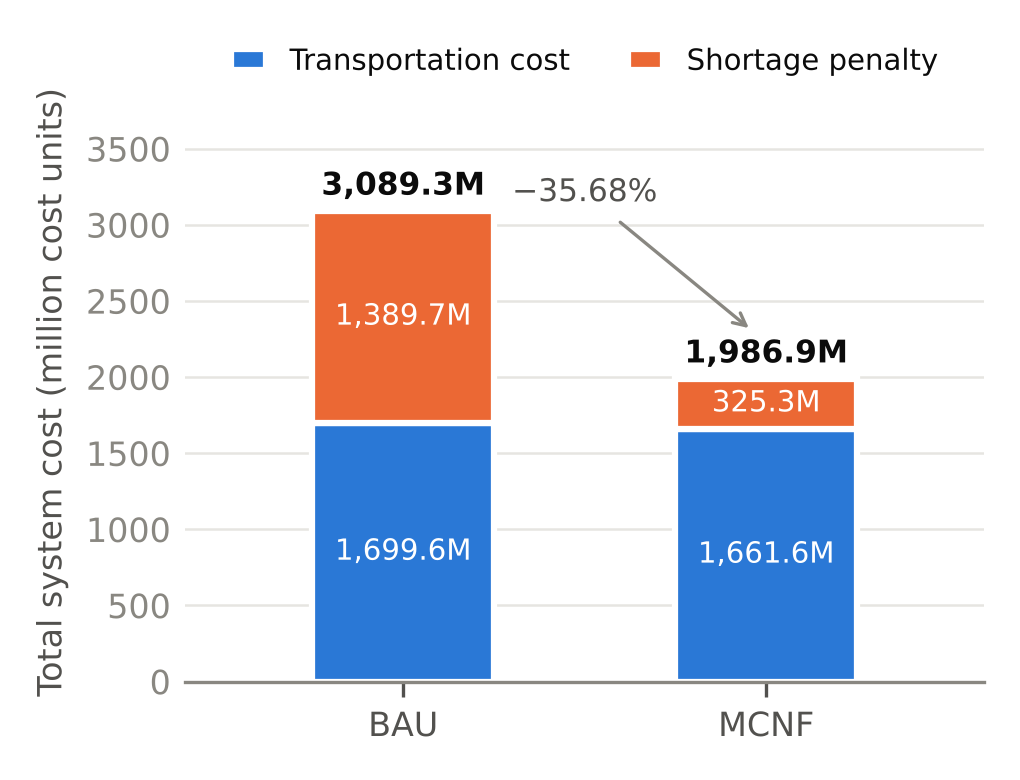
\includegraphics[width=0.75\textwidth]{fig_4_1_costs.png}
\caption{Total system cost of the BAU baseline and the optimized MCNF plan, split into transportation cost and shortage penalty.}
\end{figure}

\subsection{Macro-Scale Network Performance Metrics}
The network's operational macro-efficiency was evaluated using the standardized system metrics defined in the evaluation framework. 

\begin{itemize}
    \item \textbf{Supply Utilization (net):} The network shipped 60.65\% of the 8,141,509 t total supply (BAU: 57.45\%). The remaining 39.35\% (3,203,504 t) is unused, of which 38.37\% (3,123,777 t) is structural surplus, i.e., supply that exceeds total demand, and 0.98\% corresponds to unmet demand.
    \item \textbf{Demand Satisfaction Rate:} 98.41\% of the 5,017,732 t total demand was fulfilled (BAU: 93.21\%). The unmet 79,726.57 t (1.59\%) occurs only at Bataan\_D (palay 39,538 t; corn 11,628 t) and Zambales\_D (palay 17,195 t; corn 11,366 t). MetroDemand is fully served.
\end{itemize}

\begin{figure}[htbp]
\centering
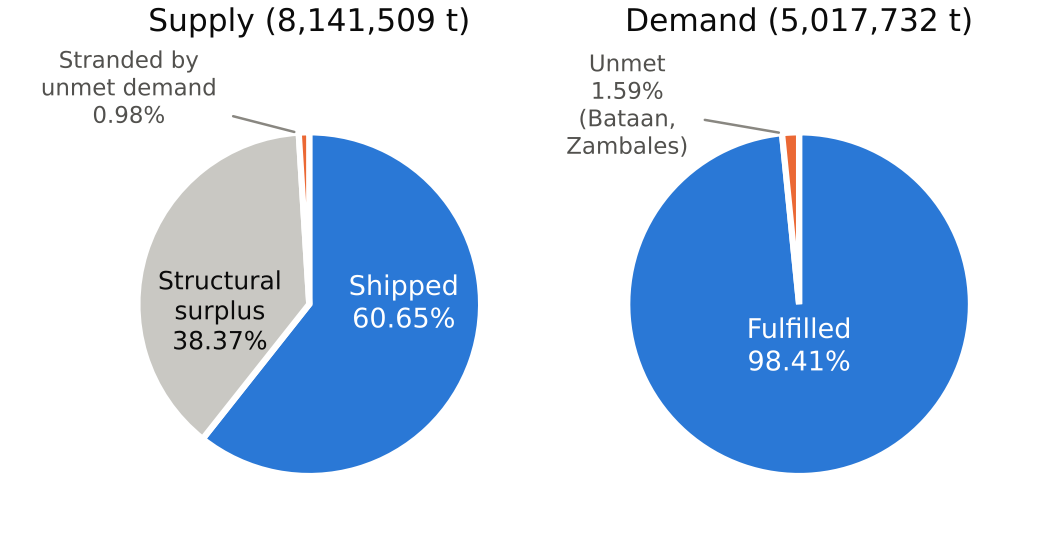
\includegraphics[width=0.9\textwidth]{fig_4_2_pies.png}
\caption{Mobilized vs.\ stranded supply (left) and fulfilled vs.\ unmet demand (right).}
\end{figure}

\subsection{Edge-Level Capacity Utilization and Bottleneck Detection}
Bottleneck detection was executed by calculating the edge utilization ratio ($\text{Utilization}_{ij} = \frac{\sum_{k \in K} x_{ij}^k}{u_{ij}}$) across all active transportation arcs. Arc segments were categorized into `Critical' ($\ge 90\%$) and `Warning' ($\ge 70\%$) zones.

Two arcs are Critical: Nueva Ecija\_S $\rightarrow$ Bulacan\_S (100.00\%) and Isabela\_S $\rightarrow$ Nueva Ecija\_S (99.68\%). One arc is in the Warning zone: Tarlac\_S $\rightarrow$ MetroDemand (70.36\%). Both critical arcs lie on the northern route that carries Cagayan, Isabela and Nueva Vizcaya supply toward Bulacan and Metro Manila. The internal local arcs (cost 20, capacity 99,000,000) stay below 1\% utilization.

\begin{table}[htbp]
\caption{Edge Capacity Utilization and Bounding Arcs}
\centering
\small
\setlength{\tabcolsep}{2.5pt}
\begin{tabular}{llrrr}
\hline
From & To & Flow (t) & Capacity (t) & Util. \\
\hline
Nueva Ecija\_S & Bulacan\_S & 1,100,000 & 1,100,000 & \textbf{100.00\%} \\
Isabela\_S & Nueva Ecija\_S & 448,552 & 450,000 & \textbf{99.68\%} \\
Tarlac\_S & MetroDemand & 773,912 & 1,100,000 & 70.36\% \\
Pangasinan\_S & Tarlac\_S & 546,174 & 900,000 & 60.69\% \\
Bulacan\_S & MetroDemand & 861,442 & 2,200,000 & 39.16\% \\
Nueva Ecija\_S & MetroDemand & 380,812 & 1,500,000 & 25.39\% \\
\hline
\end{tabular}
\end{table}

\subsection{Quantification of Regional Logistical Waste}
The total supply (8.14M t) is greater than the total demand (5.02M t) by 38.37\% which means that there is structural surplus of farm produce. Corn demonstrates this well as there is a large gap between supply (2.77M t) and demand (0.57M t). The uncapacitated model still leaves 79,726.57 t of demand unmet, the same as the capacitated model, so there is no capacity-induced shortage at the baseline capacity (0 t). The unmet demand at Bataan and Zambales is structural: neither node has incoming arcs from surplus provinces.There is increased costs due to capacity constraints. The optimal solution with capacity constraints costs 38,385,894 cost units (1.97\%) more than without them.



\begin{table}[htbp]
\caption{Largest Unused Supply per Farm Node (optimized plan)}
\centering
\small
\setlength{\tabcolsep}{2.5pt}
\begin{tabular}{llrrr}
\hline
Farm node & Commodity & Supply (t) & Unused (t) & Unused \% \\
\hline
Isabela\_S & Corn & 1,102,163 & 1,075,813 & 97.6 \\
Cagayan\_S & Corn & 594,125 & 574,169 & 96.6 \\
Cagayan\_S & Palay & 687,108 & 530,121 & 77.2 \\
Isabela\_S & Palay & 952,172 & 296,334 & 31.1 \\
Quirino\_S & Corn & 174,811 & 171,739 & 98.2 \\
Pangasinan\_S & Corn & 365,620 & 160,760 & 44.0 \\
\hline
\end{tabular}
\end{table}

\subsection{Sensitivity Analysis}
Capacity was scaled from 100\% to 40\% of its baseline value ($\lambda = 2.0$). The MCNF plan keeps unmet demand at 1.59\% down to 60\% capacity, with total cost rising 2.41\% at 70\% capacity. Shortage appears only at 50\% capacity (2.28\%) and becomes severe at 40\% (9.25\%, cost +58.9\%). BAU unmet demand rises steadily from 6.79\% to 13.88\%. A penalty sweep ($\lambda = 1.1, 1.25, 1.5, 2.0, 3.0$) left unmet demand unchanged at 79,726.57 t (1.59\%).

\begin{table}[htbp]
\caption{Capacity Sensitivity (cost units)}
\centering
\small
\setlength{\tabcolsep}{2pt}
\begin{tabular}{rrrrrr}
\hline
Cap. & MCNF cost & MCNF unmet & BAU cost & BAU unmet & Gap \\
\hline
100\% & 1,986.9M & 1.59\% & 3,089.3M & 6.79\% & 35.68\% \\
90\% & 2,002.7M & 1.59\% & 3,424.8M & 8.50\% & 41.52\% \\
80\% & 2,018.7M & 1.59\% & 3,804.3M & 10.69\% & 46.94\% \\
70\% & 2,034.7M & 1.59\% & 3,881.7M & 11.29\% & 47.58\% \\
60\% & 2,054.6M & 1.59\% & 4,049.9M & 12.46\% & 49.27\% \\
50\% & 2,206.5M & 2.28\% & 3,978.7M & 12.46\% & 44.54\% \\
40\% & 3,157.1M & 9.25\% & 4,181.7M & 13.88\% & 24.50\% \\
\hline
\end{tabular}
\end{table}

\newpage

%%%%%%%%%%%%%%%%%%%%%%%%%%%%%%%%%%%%%%%%%%%%%%%%%%%%%%%%%%%%%%%%%%%%%%%%%%%
%                      DISCUSSION AND CONCLUSION
%%%%%%%%%%%%%%%%%%%%%%%%%%%%%%%%%%%%%%%%%%%%%%%%%%%%%%%%%%%%%%%%%%%%%%%%%%%
\subsection{Interpretation of Algorithmic Flow Reallocation}
The 35.68\% reduction shows the benefit of a holistic optimization over greedy routing. This is mainly because there is a greater amount of demand met in the optimal solution. There is significantly less unmet demand under the BAU solution (6.79\%) compared to the optimal solution (1.59\%). The reduction in transportation cost was minimal (2.23\%). The higher unmet demand under BAU is likely due to its allocating shared capacity per commodity and per node, which fills some arcs to capacity before later demand nodes can use them.

Under the optimal plan, goods are routed through Nueva Ecija\_S from Isabela\_S, Nueva Vizcaya\_S, Quirino\_S and Aurora\_S. Then through Tarlac\_S and Bulacan\_S. Goods are sent through the low cost arc between Bulacan\_S and MetroDemand ($c_{ij}=124.2$) at a 39\% utilization. Tarlac\_S sends goods to MetroDemand amounting to 773,912 t (70.36\%).

\begin{figure}[htbp]
\centering
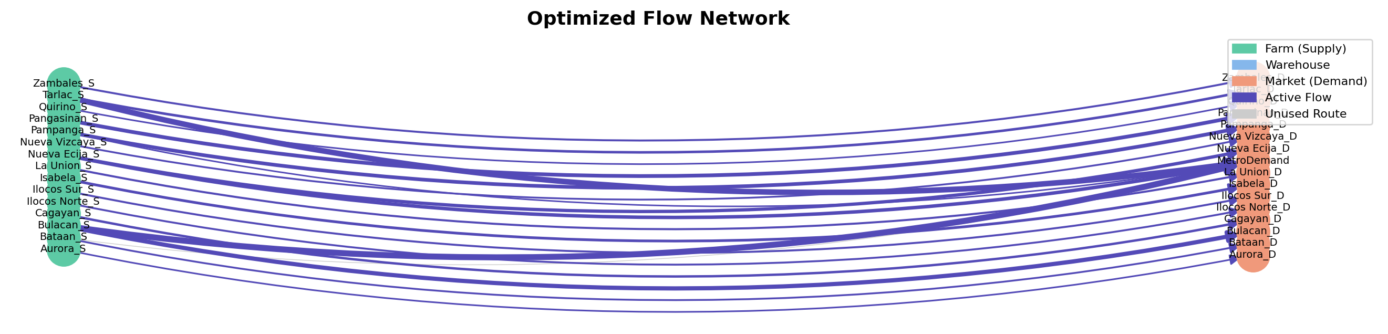
\includegraphics[width=\textwidth]{mcnf_network.png}
\caption{Optimized flow network. Edge thickness is proportional to total flow.}
\end{figure}

\subsection{Structural Causes of Unmet Demand and Unused Supply}
The model indicates that there is a demand shortage of 1.59\% and a surplus of 38.37\%. However, this is not conflicting as the surplus happens in the Northern Provinces (principally corn in Isabela, Cagayan and Quirino). The demand shortage occurs in Bataan and Zambales. The reason why there is a demand shortage is because in an uncapacitated model this will not change (79,726.57 t) as neither Bataan\_S nor Zambales\_S have any incoming arcs from the surplus nodes. Therefore, Bataan\_D and Zambales\_D can only receive supply from their own limited supply. Adding arcs to these nodes in the network is likely to eliminate the demand shortage. However increasing arc capacities would not. Whether there would be a demand shortage with more roads in the network (extra arcs such as Tarlac to Zambales) is beyond the scope of this study.

However, the costs are affected by the capacity constraint. The arcs Nueva Ecija\_S $\rightarrow$ Bulacan\_S and Isabela\_S $\rightarrow$ Nueva Ecija\_S are both at or close to full capacity (100\% and 99.68\%). This causes the optimal solution to increase by 1.97\% due to capacity constraints.

\subsection{Sensitivity Analysis and Stress Testing Results}
When scaling down arc capacity to simulate a large number of blocked roads, a 30\% reduction in capacity (70\%) creates an increase in the overall cost of the MCNF solution of 2.41\% whilst keeping the unmet demand constant at 1.59\%. The BAU solution increases unmet demand from 6.79\% to 11.29\%. The network is robust to minor disruptions due to the optimised routing around the lost capacity. The system becomes non-robust when capacity falls below approx. 60\%. At 50\% unmet demand increases to 2.28\% and at 40\% unmet demand increases to 9.25\%. The cost also increases significantly at 40\% by 58.9\%. Unmet demand is also robust to the penalty multiplier, as unmet demand remains constant between $\lambda$=1.1 and 3.0.


\section{CONCLUSION AND RECOMMENDATIONS}

\subsection{Conclusion}
In this study, a Multi-Commodity Network Flow Model was developed using Pyomo and GLPK to optimize palay and corn distribution from the Regions I, II and III to several demand nodes located in the same region and Metro Manila. Total system cost was reduced by 35.68\% from a greedy baseline distribution. Demand satisfaction increased from 93.21\% to 98.41\%. Transportation cost was reduced by 2.23\%, however, most of the savings were due to reduced shortages.

The results show that the arcs Nueva Ecija\_S to Bulacan\_S and Isabela\_S to Nueva Ecija\_S are the most heavily used arcs within the system. The unmet demand for Bataan and Zambales (1.59\%) is due to the absence of supply arcs within the model. The supply is greater than the demand for food within the model (38.37\%), so there is no need for increased farm production. However, feed and industrial demand for corn was not considered within the model. Expanding capacity on the Isabela -- Nueva Ecija -- Bulacan corridor would lower transport cost, but the benefit is modest because capacity limits raise the optimal cost by only 1.97\%. This interactive prototype can be used to help logistics and policy planning within agricultural food corridors.

% % APPENDICES

\subsection{Limitations and Recommendations for Future Work}
This model assumes flows are continuous and divisible ($x_{ij}^k \in \mathbb{R}^+$). This does not take into account the perishable products and integer restrictions in the vehicle routing problem. The arc costs do not reflect the true costs of the long haul bulk freight industry, but instead are based on a price for short haul on demand trucking. The arc capacities are also assumed and based on how many trucks can use the route. The supply and demand nodes have been aggregated at a provincial level. The demand has been restricted to human consumption of corn. Animal feed and industrial uses of corn (which contribute a large proportion of corn use) have not been modelled. This may cause the corn surplus to be overestimated. The results will also depend upon which network of 20 arcs we decide to use. Other potential road networks have not been modelled, so adding extra arcs will not increase, just maintain or decrease the optimal cost. This may change the bottlenecks and shortages within the model. The BAU baseline only uses one particular greedy heuristic, so the amount saved will depend on how it is defined.

\makereferences{references}

\doublespacing
\section{APPENDIX A. INTER-PROVINCE ARC DATA}
Table~\ref{tab:appA} lists the 20 inter-province arcs used in the model. Cost = distance $\times$ 60 $\div$ 20 t. Capacities are assumed and expressed as truck-trip equivalents.

\begin{table}[htbp]
\caption{Arc data for the 20 inter-province arcs}
\label{tab:appA}
\centering
\small
\setlength{\tabcolsep}{1.5pt}
\begin{tabular}{llrrrr}
\hline
From & To & Dist. (km) & Cost (/t) & Cap. (t/yr) & Trucks/day \\
\hline
Ilocos Norte & Ilocos Sur & 137 & 411 & 450,000 & 62 \\
Ilocos Sur & La Union & 99.3 & 298 & 450,000 & 62 \\
La Union & Pangasinan & 94.7 & 284.1 & 550,000 & 75 \\
Pangasinan & Tarlac & 71.2 & 213.6 & 900,000 & 123 \\
Pangasinan & Bulacan & 182 & 546 & 750,000 & 103 \\
Tarlac & Pampanga & 62.7 & 188.1 & 900,000 & 123 \\
Tarlac & Metro Manila & 131 & 393 & 1,100,000 & 151 \\
Zambales & Pampanga & 175 & 525 & 400,000 & 55 \\
Pampanga & Metro Manila & 79.5 & 238.5 & 1,800,000 & 247 \\
Cagayan & Isabela & 209 & 627 & 900,000 & 123 \\
Cagayan & Aurora & 197 & 591 & 450,000 & 62 \\
Isabela & Nueva Vizcaya & 153 & 459 & 750,000 & 103 \\
Isabela & Nueva Ecija & 259 & 777 & 450,000 & 62 \\
Quirino & Nueva Ecija & 206.7 & 620 & 300,000 & 41 \\
Nueva Vizcaya & Nueva Ecija & 142 & 426 & 750,000 & 103 \\
Aurora & Nueva Ecija & 243 & 729 & 450,000 & 62 \\
Nueva Ecija & Bulacan & 101 & 303 & 1,100,000 & 151 \\
Nueva Ecija & Metro Manila & 176 & 528 & 1,500,000 & 205 \\
Bulacan & Metro Manila & 41.4 & 124.2 & 2,200,000 & 301 \\
Bataan & Metro Manila & 162 & 486 & 900,000 & 123 \\
\hline
\end{tabular}
\end{table}

\section{APPENDIX B. POPULATION AND DEMAND PER DEMAND NODE}
Table~\ref{tab:appB} lists the population and annual food demand of each demand node, computed as population $\times$ per capita consumption $\div$ 1000.

\begin{table}[htbp]
\caption{Population and annual demand per demand node}
\label{tab:appB}
\centering
\small
\setlength{\tabcolsep}{3pt}
\begin{tabular}{lrrr}
\hline
Demand node & Population & Rice (t) & Corn (t) \\
\hline
Ilocos Norte  & 628,200    & 74,127.60    & 9,423.00 \\
Ilocos Sur    & 735,053    & 86,736.25    & 11,025.80 \\
La Union      & 859,561    & 101,428.20   & 12,893.42 \\
Pangasinan    & 3,235,249  & 381,759.38   & 48,528.74 \\
Cagayan       & 1,330,399  & 156,987.08   & 19,955.99 \\
Isabela       & 1,756,661  & 207,286.00   & 26,349.92 \\
Nueva Vizcaya & 506,715    & 59,792.37    & 7,600.73 \\
Quirino       & 204,798    & 24,166.16    & 3,071.97 \\
Aurora        & 237,837    & 28,064.77    & 3,567.55 \\
Bataan        & 896,684    & 105,808.71   & 13,450.26 \\
Bulacan       & 3,923,826  & 463,011.47   & 58,857.39 \\
Nueva Ecija   & 2,582,695  & 304,758.01   & 38,740.43 \\
Pampanga      & 3,115,786  & 367,662.75   & 46,736.79 \\
Tarlac        & 1,533,124  & 180,908.63   & 22,996.86 \\
Zambales      & 949,718    & 112,066.72   & 14,245.77 \\
Metro Manila  & 15,231,000 & 1,797,258.00 & 228,465.00 \\
\hline
Total         & 37,727,306 & 4,451,822.10 & 565,909.62 \\
\hline
\end{tabular}
\end{table}

\end{mainmatter}
\end{document}
